\begin{frame}{What is a game?}
	Informal definition:

	\vfill
	\begin{quotation}
		Game theory is the mathematical study of interaction among independent, self-interested agents.\\
		{\color{colornote}-- Essentials of Game Theory \cite{leyton2008essentials}}
	\end{quotation}

	\vfill
	Examples:
	\begin{enumerate}
		\item Tic-tac-toe, chess, Monopoly, etc.
		\item Economic games (includes/are included in: ecological games)
		\item Social dilemmas (PD, 'tragedy of the commons', etc.)
		\item Proof theory, model theory, etc.
		\item Machine learning
		\item \textbf{etc.}
	\end{enumerate}
\end{frame}

\begin{frame}{Representing games}
	\vfill
	\begin{enumerate}
		\item \textbf{Normal form}:
		A set of \textbf{players} $P$, an indexed set of \textbf{actions} $A : P \to \Set$, a \textbf{utility function}
		$u : \prod_{p \in P} A\; p \to (P \to R)$

		\item \textbf{Extensive form}:
		A set of \textbf{players} $P$, a \textbf{tree} representing the unfolding of the game. Nodes are assigned to players and grouped in \textbf{information sets}. Branches are called \textbf{moves}. A \textbf{utility vector} assigned to each leaf.
	\end{enumerate}

	\vfill
	\begin{center}
		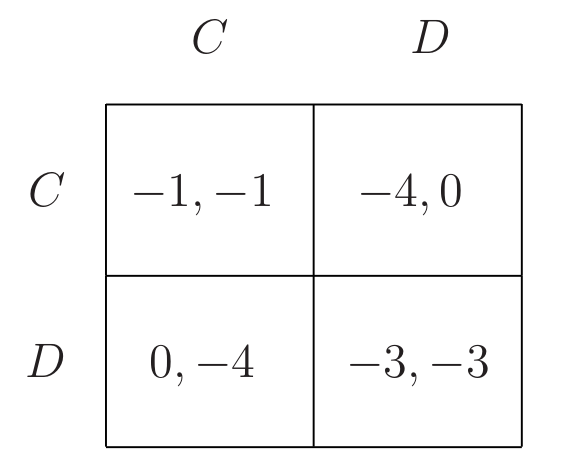
\includegraphics[width=.4\textwidth]{figures/pd_norm.png}
		\qquad
		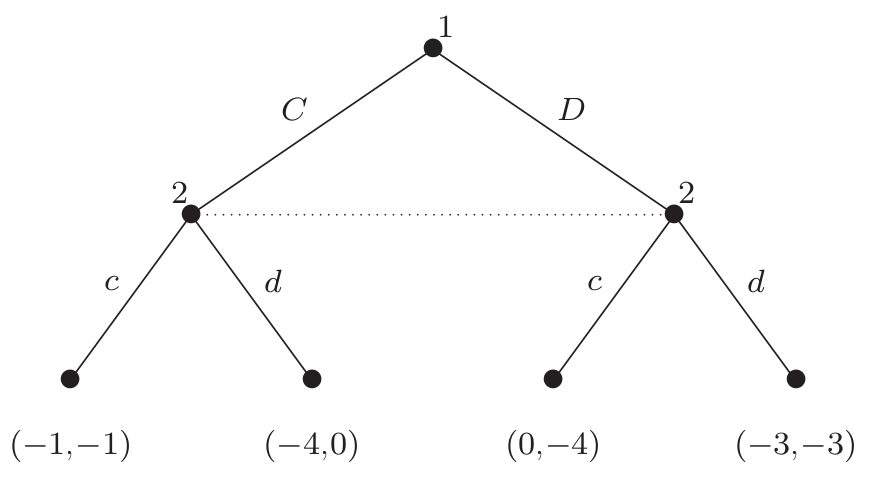
\includegraphics[width=.5\textwidth]{figures/pd_ext.png}
	\end{center}
\end{frame}

\begin{frame}{Extensive $\to$ normal}
	One can always convert an extensive form game into normal form:

	\hfill
	\begin{enumerate}
		\item Define
		\begin{equation*}
			A\; p = \sum_{x \in \text{$p$'s nodes}} \text{moves at $x$}
		\end{equation*}
		\item Define
		\begin{eqalign*}
			u(\text{action profile $a_1, \ldots, a_n$}) &=
			u(\text{path $a_1, \ldots, a_n$})\\
			&= \text{payoff at the end of the path}.
		\end{eqalign*}
	\end{enumerate}

	\vfill
	The converse is not always possible since normal-form games have too little structural information.
\end{frame}

\begin{frame}{Solving games}
	\textbf{Pre-formal definition}: A \textbf{solution concept} is a notion of `optimality' for ways to play a game.

	A 'way to play' for a player $p \in P$ is called \textbf{strategy}:
	\begin{equation*}
		\Omega\; p = \prod_{x \in \text{$p$'s nodes}} \text{moves at $x$}
	\end{equation*}
	Compare it with
	\begin{equation*}
		A\; p = \sum_{x \in \text{$p$'s nodes}} \text{moves at $x$}
	\end{equation*}

	\textbf{Key difference}: strategies are a \textbf{comprehensive plan of action}: for each \textbf{state} of the game, no matter how unlikely, we plan an \textbf{action}.

	A choice of strategy for each player is a \textbf{strategy profile}:
	\begin{equation*}
		S = \prod_{p \in P} \Omega\; p
	\end{equation*}
\end{frame}

\begin{frame}{Nash equilibrium}
	The most important (and general) solution concept is \textbf{Nash equilibrium}:

	\vfill
	\begin{definition}
		A strategy profile $s \in S$ is a Nash equilibrium if no player has interest in unilaterally deviating its strategy.
	\end{definition}

	\vfill
	e.g. for utility-maximizing players:

	\begin{equation*}
		\forall p \in P,\, \forall s'_p \in \Omega\; p \quad u_i(s[s_p/s'_p]) \leq u_p(s)
	\end{equation*}

	\vfill
	It's not the only one: SGP, ESS, $\epsilon$-Nash, trembling hand, etc.

	Afaik, all are \textbf{refinements} of Nash.
\end{frame}

\begin{frame}{Nash equilibrium: example}
	\begin{center}
		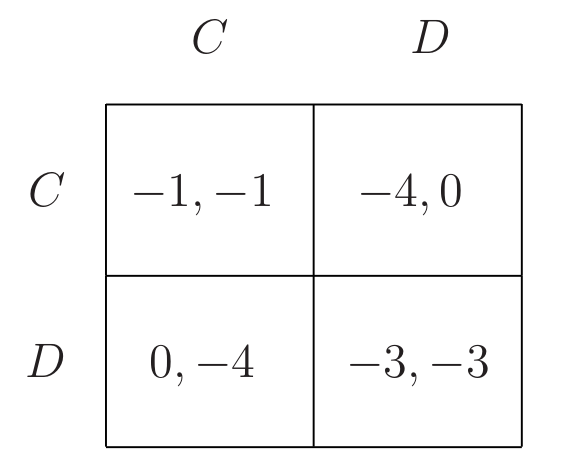
\includegraphics[width=.6\textwidth]{figures/pd_norm.png}
	\end{center}
\end{frame}

\begin{frame}{Pros and cons}
	Problems with classical game theory:
	\begin{enumerate}
		\item Games are treated \textbf{monolithically}
		\item Stuck in \textbf{early 20th century mathematical language}
		\item Denotations are quite disappointing: normal form is too opaque, extensive form is too... extended
	\end{enumerate}

	Open games are a proposed improvement:
	\begin{enumerate}
		\item Games are defined \textbf{compositionally}, including \textbf{equilibria}
		\item Mathematically more sophisticated (grounded in \textbf{category theory})
		\item Denoted by \textbf{string diagrams}: halfway between normal and extensive form
	\end{enumerate}

	It follows the ACT tradition of `opening up' systems: \emph{always consider a system as part of an environment it interacts non-trivially with}
\end{frame}
